%%
%% Author: novitoll
%% 2/24/18
%%

% Preamble
\documentclass[11pt]{article}

% Packages
\usepackage{amsmath}
\usepackage{graphicx}
\DeclareMathOperator*{\argmax}{arg\,max}
\DeclareMathOperator{\atantwo}{atan2}

\title{CVT: Lecture 3}
\date{2018-02-25}
\author{Novitoll}

\graphicspath{ {code/} }

% Document
\begin{document}
    \maketitle
    \pagenumbering{arabic}

    \section{Projection peaks}

    Given calculated projection of text lines in the input image,
    then you want to find maxima of them:

    \begin{align}
        y_{\text{bm}} = \argmax{p_y(y)}
    \end{align}

    In this case, first we need to find left and right minimum per some coefficient of the peak:

    \begin{align}
        y_{\text{b0}} = \max_{y_0 < y < y_{\text{bm}}}(y|p_y(y) <= c_y * p_y(y_{\text{bm}})) \\
        y_{\text{b1}} = \min_{y_0 < y < y_{1}}(y|p_y(y) <= c_y * p_y(y_{\text{bm}}))
    \end{align}

    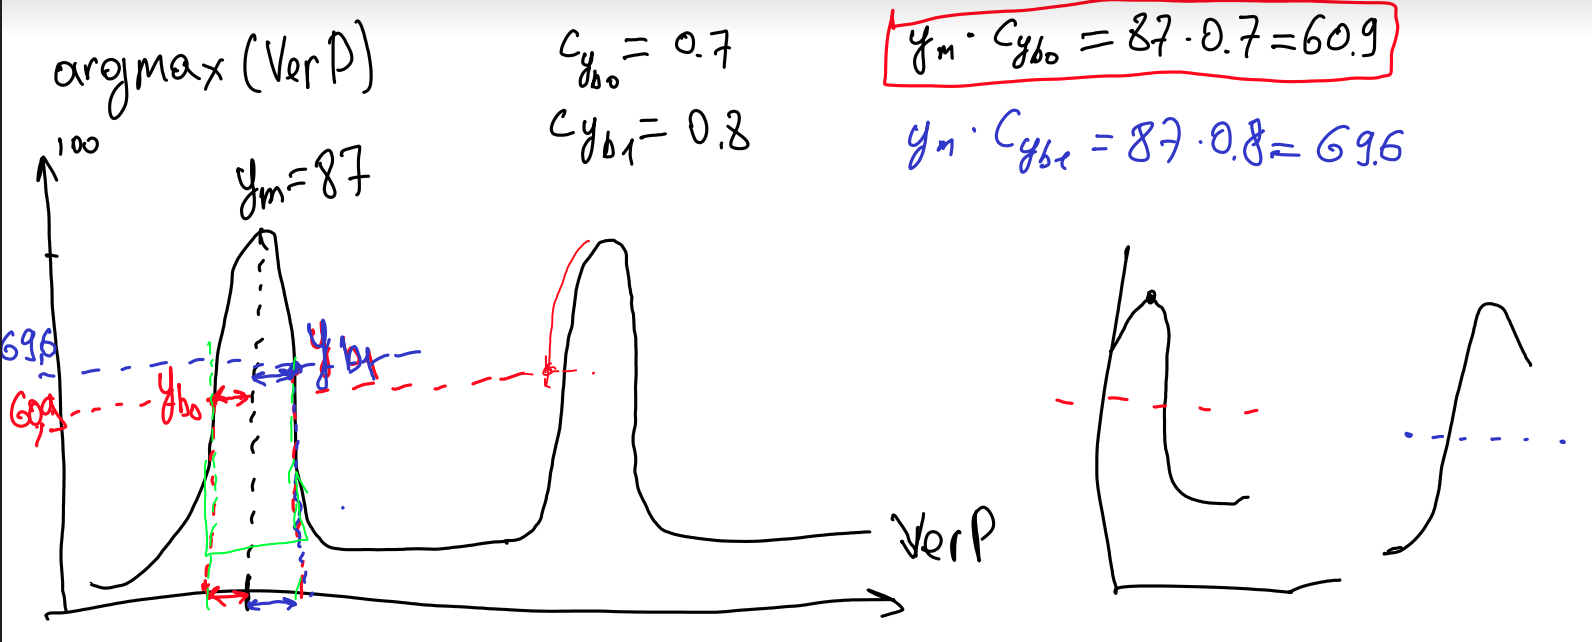
\includegraphics[scale=0.2]{peaks}

    \section{Sobel gradients magnitude}

    Given calculated with Sobel filter gradients of X and Y axis,
    you can combine them, deriving
    \begin{itemize}
        \item magnitude - $\sqrt{x^2 + y^2}$
        \item gradient angle - $\atantwo(y, x)$
    \end{itemize}

    \section{HOG}

    HOG (Histogram of oriented gradients) can be used for generating features (Sobel X, Y gradients magnitude and angle)
    for machine learning model (Was presented in CVPR 2005 with SVM usage for object detection).

    HOG requires params as:
    \begin{itemize}
        \item cell\_size
        \item orientation
        \item block\_size
    \end{itemize}

    , where orientation is integer (in opencv2) of N-dimensionality of axis.

    HOG can be also used as normalization for rotation and region (template) detection, e\.g\. for normalization -
    can be used to analyze the rotation effect (histogram will be shifted but magnitude values remain same),
    for template detection - take the tiny part of the image, get its HOG, and you can find its position in the image,
    comparing template HOG with image's testing region HOG

    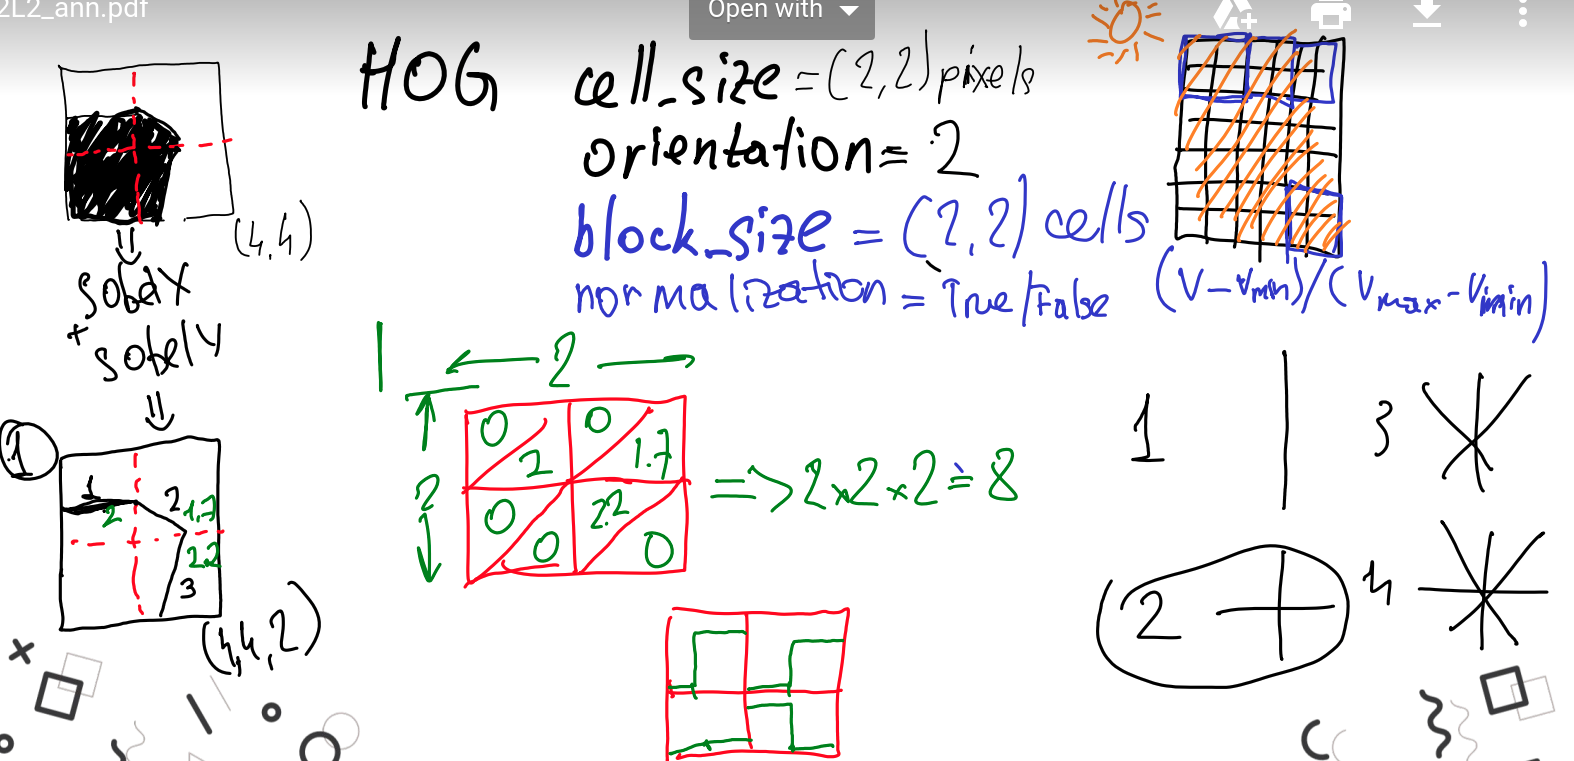
\includegraphics[scale=0.2]{hog}
    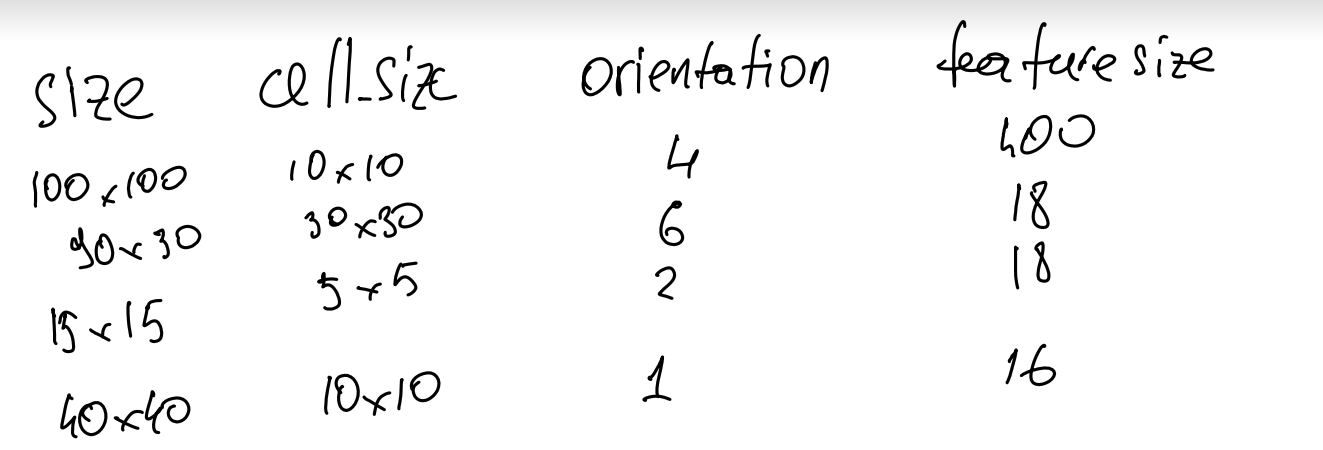
\includegraphics[scale=0.2]{hog_feature}
    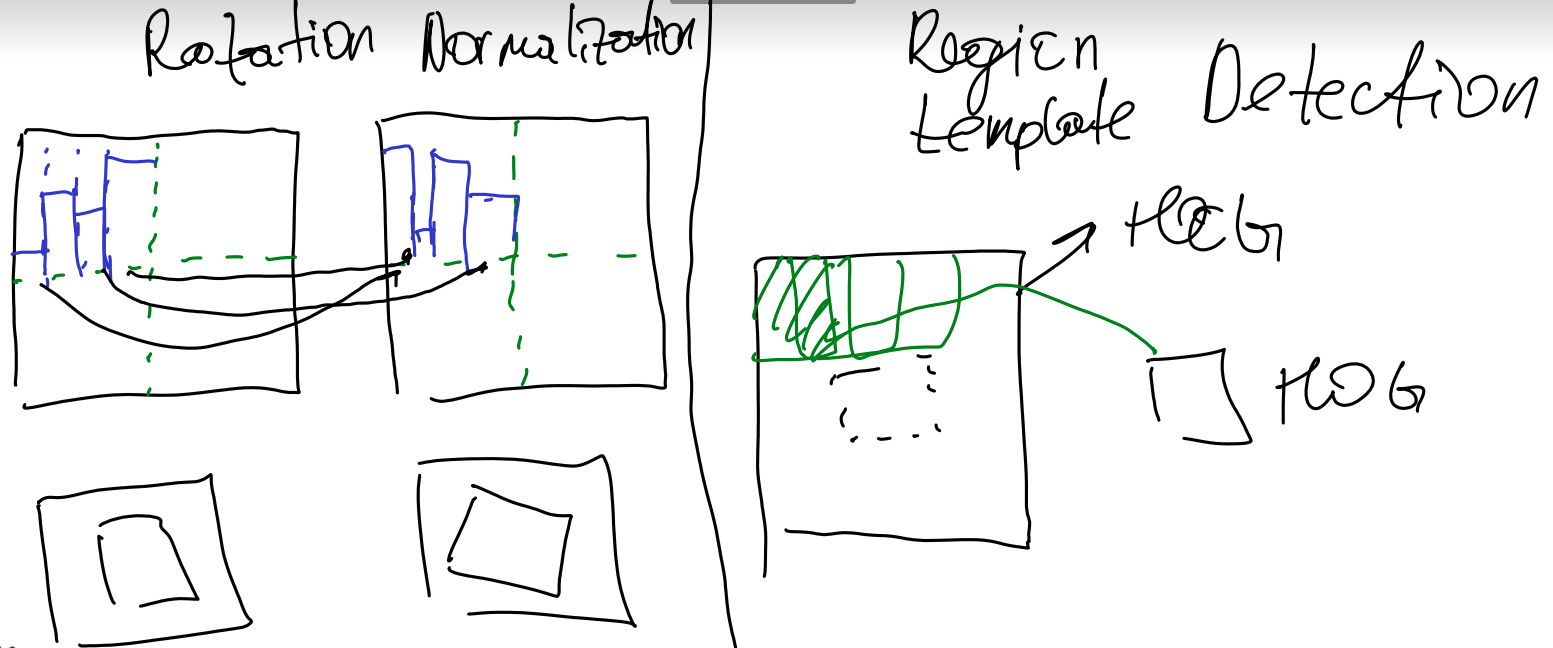
\includegraphics[scale=0.2]{hog_usage}

\end{document}